En el siguiente capítulo se desarrolla la estructura organizativa del sistema sanitario de Castilla y León a lo largo de todos los estratos además de ofrecer algunos datos relevantes sobre los servicios que se ofrecen a la población.

\section{Perfil de la organización}

El Área de Salud Valladolid Oeste (ASVAO) presta asistencia sanitaria a la población de aproximadamente la mitad de la provincia de Valladolid, la situada geográficamente en la zona oeste. Esta atención sanitaria se provee en sus dos niveles asistenciales: Atención Primaria (con 17 Zonas Básicas de Salud) y Atención Hospitalaria (con el Hospital Universitario Rio Hortega y el Centro de Especialidades de Arturo Eyries).

El Área de Salud Valladolid Oeste (ASVAO) forma parte del Sistema Público de Salud de Castilla y León, el cual comprende el conjunto de actuaciones y recursos públicos de la Administración Sanitaria de la Comunidad Autónoma y de las Corporaciones Locales, cuya finalidad es la promoción y protección de la salud en todos sus ámbitos, la prevención de la enfermedad, la asistencia sanitaria y la rehabilitación, todo ello bajo una perspectiva de asistencia sanitaria integral (Ley 8/2010, de 30 de agosto, de ordenación del sistema de salud de Castilla y León).

El Hospital Universitario Río Hortega fue inaugurado como Centro Hospitalario el 24 de Julio de 1953. En ese momento disponía de 310 camas y 72 cunas. Tras más de 50 años ubicado en pleno centro (cerca de la plaza de San Pablo), se trasladó a un nuevo edificio en el año 2008, esta vez situado a las afueras de la ciudad, en el barrio de las Delicias. En estos momentos cuenta con 640 camas instaladas y se configura como un hospital general, universitario y de tercer nivel. Además de prestar atención sanitaria al Área de Salud Valladolid Oeste, para determinadas prestaciones actúa como “Servicio de Referencia”, ampliando su cobertura a toda la provincia de Valladolid o incluso a varias provincias limítrofes. En algunos casos presta servicio a toda la Comunidad Autónoma.

En BOCYL de 24 de octubre de 2008, según ACUERDO 111/2008 de 23 de octubre de la Junta de Castilla y León, se reestructura el Área de Salud de Valladolid Oeste y el Área de Salud de Valladolid Este.

La apertura del nuevo Hospital Universitario Río Hortega, que cambia de ubicación, hace necesaria la adaptación del mapa sanitario del Área de Salud de Valladolid Oeste, pasando las Z.B.S. Centro Gamazo, Z.B.S. la Victoria, Z.B.S. Rural I, Z.B.S. Cigales a pertenecer al Área Este de Valladolid y las Z.B.S. Delicias I y Z.B .S. Delicias II pasan a pertenecer al Área Oeste de Valladolid.

Al frente de la organización se han sucedido los siguientes nombramientos en los últimos años: Por Orden SAN/465/2012 de 18 de junio se nombró Gerente de Atención Especializada a D. Alfonso Montero Moreno, posteriormente por resolución de 15 de febrero de 2012 del Gerente Regional de Salud se acumularon las funciones de Gerente de Atención Primaria a las de Gerente de Atención Hospitalaria. El 18 de julio de 2015 fue nombrado como Gerente de Atención Primaria D. Eduardo García Prieto. Por último en el año 2018 a través de Orden SAN/901/2018 de 10 de agosto se nombró Gerente de Atención Especializada a D. José Miguel García Vela.

A partir del mes de marzo de 2017 todo el personal de la Gerencia de Atención Primaria se integró a trabajar en las instalaciones del HURH junto a de los diferentes servicios correspondientes.

\section{Cartera de servicios}

El Área de Salud Valladolid Oeste (ASVAO) es la organización a la que se adscribe todo el dispositivo sanitario del Área, compuesto por los 17 Centros de A. Primaria y por el Hospital Universitario Río Hortega. El objetivo primordial de esta organización es la prestación de asistencia sanitaria a la población del Área Oeste de Valladolid, tanto en Atención Primaria, enAtención Hospitalaria como en Atención Sociosanitaria (esta última compartida con la Gerencia Regional de Servicios Sociales).

La Atención Primaria es el nivel básico e inicial de atención, que garantiza la globalidad y continuidad de ésta a lo largo de la vida del paciente, actuando como gestor y coordinador de casos y regulador de flujos. Comprende actividades de promoción de la salud, educación sanitaria, prevención de la enfermedad, asistencia sanitaria, mantenimiento y recuperación de la salud, así como la rehabilitación física y el trabajo social.

La Atención Hospitalaria comprende las actividades asistenciales, diagnósticas, terapéuticas y de rehabilitación y cuidados, así como aquellas de promoción de la salud, educación sanitaria y prevención de la enfermedad, cuya naturaleza aconseja que se realicen en ese nivel. La Atención Hospitalaria garantizará la continuidad de la atención integral al paciente, una vez superadas las posibilidades de la Atención Primaria y hasta que aquel pueda reintegrarse en dicho nivel. Prestará además, servicios de hospitalización en régimen de internamiento, asistencia especializada en consultas, hospital de día (médico y quirúrgico), atención paliativa a enfermos terminales, salud mental y rehabilitación en pacientes con déficit funcional recuperable.

La Atención Sociosanitaria comprende el conjunto de cuidados destinados a aquellos enfermos, generalmente crónicos, que por sus especiales características pueden beneficiarse de la actuación simultánea y sinérgica de los servicios sanitarios y sociales para aumentar su autonomía, paliar sus limitaciones o sufrimientos y facilitar su reinserción social. En el ámbito sanitario, la Atención Sociosanitaria comprenderá los cuidados sanitarios de larga duración, la atención sanitaria a la convalecencia y la rehabilitación en pacientes con déficit funcional recuperable.

\subsection{Servicios en Atención Primaria}

La cartera de servicios en Atención Primaria de Valladolid Oeste está compuesta por:

\begin{table}[H]
    \centering
    \begin{tabular}{l}
        \toprule
        Servicios                                             \\
        \midrule
        Medicina familiar y comunitaria                       \\
        Pediatría                                             \\
        Enfermería                                            \\
        Unidad de salud bucodental                            \\
        Unidad de atención a la mujer                         \\
        Fisioterapia                                          \\
        Extracciones laboratorio                              \\
        Radiología                                            \\
        Urgencias                                             \\
        Asistemcia social                                     \\
        Cirugía menor                                         \\
        Diagnóstico ecográfico                                \\
        Farmacia                                              \\
        Unidad administrativa de citas y atención al paciente \\
        Prevención y promoción de la salud                    \\
        \bottomrule
    \end{tabular}
    \caption{Cartera de servicios en atención primaria}
\end{table}

Existe un amplio capítulo de actuaciones dirigidas a la Prevención y Promoción de la Salud, en el que se incluyen, entre otros, programas de vacunación infantil, programas de vacunación en el adulto, desarrollo de actividades preventivas en el adulto sano, prevención de obesidad infantil, atención a pacientes crónicos (hipertensión arterial, dislipemias, diabetes, EPOC, etc.), atención al paciente crónico pluripatológico complejo, prevención precoz de cáncer de mama, de colon, deshabituación tabáquica, atención a pacientes ancianos de riesgo o en situación terminal, violencia de género, etc.

\subsection{Servicios en Atención Especializada}

En la siguiente tabla se refleja la Cartera de Servicios Básica del Hospital Universitario Río Hortega.

\begin{table}[H]
    \centering
    \begin{tabular}{cl}
        \toprule
        \multirow{16}{*}{Servicios Médicos}                 & Alergología                          \\
                                                            & Aparato Digestivo                    \\
                                                            & Cardiología                          \\
                                                            & Endocrinología y Nutrición           \\
                                                            & Geriatría                            \\
                                                            & Hematología y Hemoterapia            \\
                                                            & Medicina Intensiva                   \\
                                                            & Medicina Interna                     \\
                                                            & Nefrología                           \\
                                                            & Neumología                           \\
                                                            & Neurología                           \\
                                                            & Oncología médica                     \\
                                                            & Pediatría                            \\
                                                            & Psiquiatría                          \\
                                                            & Rehabilitación                       \\
                                                            & Reumatología                         \\
        \midrule
        \multirow{10}{*}{Servicios   Quirúrgicos}           & Anestesiología y Reanimación         \\
                                                            & Cirugía General y Digestiva          \\
                                                            & Cirugía Oral y Maxilofacial          \\
                                                            & Cirugía Plástica Reparadora          \\
                                                            & Dermatología Medicoquirúrgica        \\
                                                            & Neurocirugía                         \\
                                                            & Obstetricia Y Ginecología            \\
                                                            & Oftalmología                         \\
                                                            & Traumatología y Cirugía Ortopédica   \\
                                                            & Urología                             \\
        \midrule
        \multirow{7}{*}{Servicios   Centrales Diagnósticos} & Urgencias                            \\
                                                            & Admisión y Documentación Clínica     \\
                                                            & Farmacia Hospitalaria                \\
                                                            & Farmacología Clínica                 \\
                                                            & Medicina del Trabajo                 \\
                                                            & Medicina Preventiva y Salud Pública  \\
                                                            & Radiofísica y Protección Radiológica \\
        \midrule
        \multirow{7}{*}{Servicios   Especiales}             & Cuidados Paliativos                  \\
                                                            & Atención a Domicilio                 \\
                                                            & Unidad del Dolor                     \\
                                                            & Transplante de Médula Ósea Autólogo  \\
                                                            & Transplante de Médula Ósea Alogénico \\
                                                            & Hepatología                          \\
                                                            & Transplante Hepático y Hepatorrenal  \\
        \midrule
        \multirow{5}{*}{Servicios Técnicos}                 & Unidad de Calidad                    \\
                                                            & Unidad de Docencia                   \\
                                                            & Unidad de Formación Continuada       \\
                                                            & Unidad de Apoyo a la Investigación   \\
                                                            & Unidad de Comunicación Interna       \\
        \bottomrule
    \end{tabular}
    \caption{Cartera de servicios en atención especializada}
\end{table}

\section{Localización de la sede principal}

La sede principal del Área de Salud Valladolid Oeste (ASVAO) se encuentra ubicada en el Hospital Universitario Río Hortega, que se localiza en la calle Dulzaina Nº2 de la ciudad de Valladolid.

\begin{figure}[H]
    \centering
    \begin{subfigure}[H]{0.45\textwidth}
        \centering
        \includegraphics*[width=\textwidth]{img/mapa-comunidad.png}
        \caption{Castilla y León}
    \end{subfigure}
    \hfill
    \begin{subfigure}[H]{0.45\textwidth}
        \centering
        \includegraphics*[width=\textwidth]{img/mapa-provincia.png}
        \caption{Valladolid provincia}
    \end{subfigure}
    \hfill
    \begin{subfigure}[H]{0.45\textwidth}
        \centering
        \includegraphics*[width=\textwidth]{img/mapa-ciudad.png}
        \caption{Valladolid municipio}
    \end{subfigure}
    \hfill
    \begin{subfigure}[H]{0.45\textwidth}
        \centering
        \includegraphics*[width=\textwidth]{img/mapa-hospital.png}
        \caption{Hospital Universitario Río Hortega}
    \end{subfigure}
\end{figure}

\section{Mercado servido}

El Área de Salud Valladolid Oeste da cobertura asistencial principalmente a su área de referencia. También es referente en algunos servicios sanitarios para las Áreas de Salud de Valladolid Este, Segovia, Palencia, Burgos y Soria.

En algunas prestaciones sanitarias (grandes quemados, cirugía oncológica peritoneal, trasplante hepático, etc.) es referente para toda la Comunidad Autónoma.

\begin{table}[H]
    \centering
    \begin{tabular}{lrrr}
        \toprule
        Tramos & Hombres   & Mujeres   & TOTAL     \\
        \midrule
        0-4    & 36.946    & 35.037    & 71.983    \\
        5-9    & 46.956    & 43.96     & 90.916    \\
        10-14  & 51.88     & 48.892    & 100.772   \\
        15-19  & 50.751    & 48.621    & 99.372    \\
        20-24  & 52.015    & 50.543    & 102.558   \\
        25-29  & 55.643    & 52.816    & 108.459   \\
        30-34  & 60.369    & 59.183    & 119.552   \\
        35-39  & 71.588    & 70.903    & 142.491   \\
        40-44  & 87.788    & 86.829    & 174.617   \\
        45-49  & 91.022    & 89.775    & 180.797   \\
        50-54  & 91.527    & 91.727    & 183.254   \\
        55-59  & 91.86     & 91.072    & 182.932   \\
        60-64  & 85.689    & 84.138    & 169.827   \\
        65-69  & 69.763    & 68.877    & 138.64    \\
        70-74  & 60.221    & 64.433    & 124.654   \\
        75-79  & 49.186    & 58.037    & 107.223   \\
        80-84  & 35.301    & 49.78     & 85.081    \\
        85-89  & 28.726    & 47.49     & 76.216    \\
        90-94  & 12.641    & 26.518    & 39.159    \\
        95-100 & 3328      & 9451      & 12.779    \\
        \textbf{TOTAL}  & \textbf{1.133.200} & \textbf{1.178.082} & \textbf{2.311.282}  \\
        \bottomrule
        \end{tabular}
        \caption{Población por tramos quinquenales y sexo en el año 2020}
\end{table}

\begin{figure}[H]
    \centering
    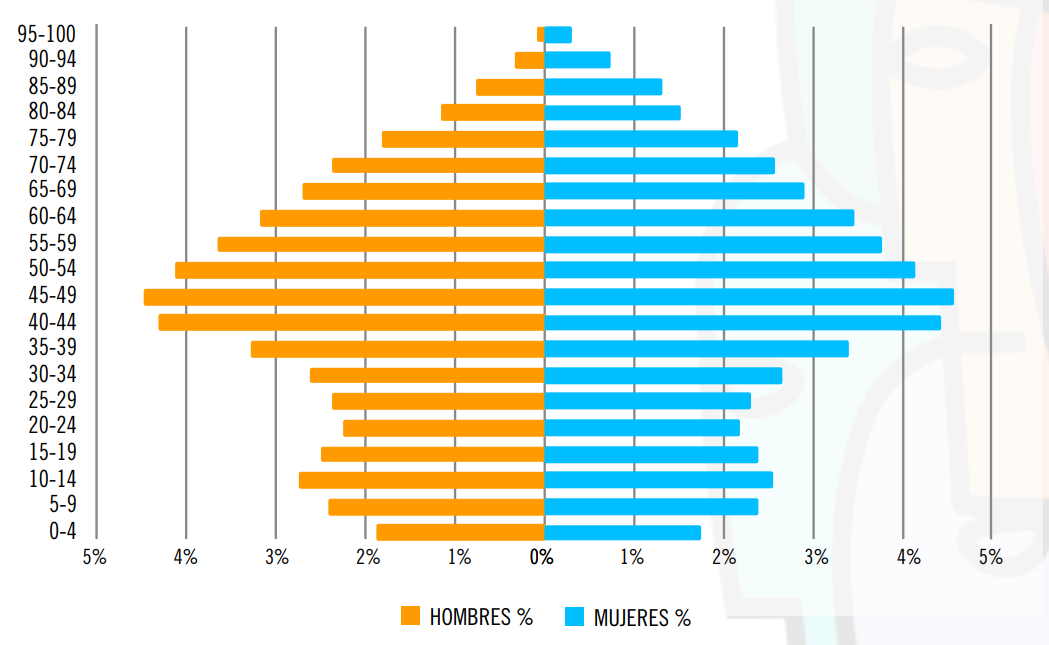
\includegraphics[width=\textwidth]{img/piramide-poblacion.png}
    \caption{Pirámide de población del Área de Salud Valladolid Oeste}
\end{figure}

Dentro de la Atención Primaria tenemos las Zonas Básicas de Salud mostradas en la siguiente tabla.

\begin{table}[H]
    \centering
    \begin{tabular}{cll}
        \toprule
        \multicolumn{2}{c}{Zonas   Básicas de Salud} & Centro de Salud                                      \\
        \midrule
        \multirow{8}{*}{Urbanas}                     & ZBS Arturo Eyries       & CS Arturo Eyries           \\
                                                     & ZBS Campo Grande        & CS Campo Grande            \\
                                                     & ZBS Esperanto           & CS Plaza del Ejército      \\
                                                     & ZBS Huerta del Rey      & CS Huerta del Rey          \\
                                                     & ZBS Parquuesol          & CS Parquesol               \\
                                                     & ZBS Valladolid Sur      & CS Parque Alameda-Covaresa \\
                                                     & ZBS Delicias I          & CS Delicias I              \\
                                                     & ZBS Delicias II         & CS Delicias II             \\
        \midrule
        \multirow{11}{*}{Rurales}                    & ZBS Laguna de Duero     & CS Laguna de Duero         \\
                                                     & ZBS Tordesillas         & CS Tordesillas             \\
                                                     & ZBS Mayorga             & CS Mayorga                 \\
                                                     & ZBS Medina de Rioseco   & CS Medina de Rioseco       \\
                                                     & ZBS Mayorga             & CS Mayorga                 \\
                                                     & ZBS Medina de Rioseco   & CS Medina de Rioseco       \\
                                                     & ZBS Mota del Marqués    & CS Mota del Marqués        \\
                                                     & ZBS Pisuerga            & CS Pisuerga                \\
                                                     & ZBS Valladolid Rural II & CS Zaratán                 \\
                                                     & ZBS Villafrechós        & CS Villafrechós            \\
                                                     & ZBS Villalón            & CS Villalón                \\
        \bottomrule
    \end{tabular}
    \caption{Relación de Zonas Básicas de Salud y Centros de Salud}
\end{table}

El Hospital Universitario Río Hortega es un hospital de tercer nivel y como tal tiene Servicios y Técnicas que son de referencia para otras áreas de la Comunidad Autónoma. A continuación se describen las áreas y los servicios o técnicas con los que el hospital actúa como centro de referencia en dichas áreas (según Orden SAN/1288/2010, de 16 de septiembre, por la que se desarrolla la ordenación y los centros y servicios de referencia en Atención Hospitalaria en la Comunidad de Castilla y León).

\begin{table}
    \centering
    \begin{tabular}{cl}
        \toprule
        Áreas de Referencia                                      & Servicios de Referencia              \\
        \midrule
        \multirow{6}{*}{Área de Salud   Valladolid Este}         & Cirugía Maxilofacial                 \\
                                                                 & Cirugía Plástica y Reparadora        \\
                                                                 & Alergología                          \\
                                                                 & Implante Coclear                     \\
                                                                 & Transplante de Médula Ósea Alogénico \\
                                                                 & Transplante de Médula Ósea Autólogo  \\
        \midrule
        \multirow{2}{*}{Área de Salud de   Ávila}                & Cirugía Plástica y Reparadora        \\
                                                                 & Implante Coclear                     \\
        \midrule
        \multirow{2}{*}{Área de Salud de   Burgos}               & Cirugía Maxilofacial                 \\
                                                                 & Implante Coclear                     \\
        \midrule
        \multirow{6}{*}{Área de Salud de   Palencia}             & Cirugía Bariátrica                   \\
                                                                 & Cirugía Maxilofacial                 \\
                                                                 & Cirugía Plástica y Reparadora        \\
                                                                 & Implante Coclear                     \\
                                                                 & Neurocirugía                         \\
                                                                 & Transplante de Médula Ósea Autólogo  \\
        \midrule
        \multirow{5}{*}{Área de Salud de   Segovia}              & Cirugía Bariátrica                   \\
                                                                 & Cirugía Maxilofacial                 \\
                                                                 & Cirugía Plástica y Reparadora        \\
                                                                 & Implante Coclear                     \\
                                                                 & Neurocirugía                         \\
        \midrule
        \multirow{3}{*}{Área de Salud de   Soria}                & Cirugía Maxilofacial                 \\
                                                                 & Implante Coclear                     \\
                                                                 & Transplante de Médula Ósea Autólogo  \\
        \midrule
        \multirow{2}{*}{Comunidad Autónoma   de Castilla y León} & Transplante Hepático                 \\
                                                                 & Unidad de Grandes Quemados           \\
        \bottomrule
    \end{tabular}
    \caption{Áreas de en las que el hospital es centro de referencia}
\end{table}

\section{Tamaño de la organización}

El Área de Salud Valladolid Oeste dispone de dos centros de gasto diferenciados y el 100\% de sus recursos provienen de la Consejería de Sanidad de Castilla y León. En las tablas \ref{tab:gastos-primaria} y \ref{tab:gastos-especializada} se muestran los presupuestos anuales del Área de Salud Valladolid Oeste diferenciando Atención Primaria y Hospitalaria.

\begin{table}
    \centering
    \begin{tabular}{lrrr}
        \toprule
        Año                              & 2016              & 2017              & 2018              \\
        \midrule
        Inversiones                      & 260317            & 353879            & 293654            \\
        Compras a proveedores            & 2054867           & 2141010           & 2157458           \\
        \textbf{TOTAL COMPRAS}           & \textbf{2315184}  & \textbf{2494889}  & \textbf{2451112}  \\
        \midrule
        Productos farmacéuticos          & 1349              & 1488              & 1488              \\
        Material sanitario               & 894527            & 980114            & 943458            \\
        Gastos externos                  & 1395160           & 1423618           & 1354330           \\
        Otros gastos de explotación      & 1158991           & 1159408           & 1212512           \\

        \textbf{TOTAL G. FUNCIONAMIENTO} & \textbf{3450027}  & \textbf{3564628}  & \textbf{3511788}  \\
        \midrule
        Gastos de personal               & 39835467          & 41112893          & 42048766          \\
        \textbf{TOTAL G. EXPLOTACIÓN}    & \textbf{43285494} & \textbf{44677521} & \textbf{45560554} \\
        \bottomrule
    \end{tabular}
    \caption{Distribución de gastos de Atención Primaria en euros}
    \label{tab:gastos-primaria}
\end{table}

\begin{table}
    \centering
    \begin{tabular}{lrrr}
        \toprule
        Año                              & 2016               & 2017               & 2018               \\
        \midrule
        Inversiones                      & 1861010            & 2989204            & 1415588            \\
        Compras a proveedores            & 78436457           & 83637670           & 93502901           \\
        \textbf{TOTAL COMPRAS}           & \textbf{80297467}  & \textbf{86626874}  & \textbf{94918489}  \\
        \midrule
        Productos farmacéuticos          & 35733953           & 39290752           & 46043592           \\
        Material sanitario               & 28171052           & 29314685           & 31564066           \\
        Gastos externos                  & 6685813            & 6805173            & 6557567            \\
        Otros gastos de explotación      & 15006676           & 15448892           & 16072760           \\
        \textbf{TOTAL G. FUNCIONAMIENTO} & \textbf{85597494}  & \textbf{90859502}  & \textbf{100237985} \\
        \midrule
        Gastos de personal               & 117863479          & 120592213          & 123511681          \\
        \textbf{TOTAL  EXPLOTACIÓN}      & \textbf{203460973} & \textbf{211451715} & \textbf{223749666} \\
        \bottomrule
    \end{tabular}
    \caption{Distribución de gastos de Atención Especializada en euros}
    \label{tab:gastos-especializada}
\end{table}